

\setstretch{1.}


\paragraph{Commentaire sur le titre}
On peut laisser encore plus de place au titre et aux indications de base: diplôme, cours, nom de l'enseignement, année, etc ... On peut ajouter le nom de l'enseignant.

Les informations peuvent être données sur une page spéciale, la première. On peut alors y ajouter une figure illustrant le travail effectué. Toujours  rester sobre
dans la présentation du titre.

\rouge{les informations ci-dessus sont obligatoires. Dans le document, le texte en gris doit être modifié pour coller au contexte.} 
 


\paragraph{Résumé}
Dans ce TP est présentée la démarche pour effectuer des simulations ...
La méthode et les résultats sont décrits et discuter.
\textit{Puis ajouter un important résultat du TP.}

\rouge{La résumé est optionnel pour un TP, il peut être rédigé en anglais.
Pour un TP 5 à 10 lignes sont suffisantes.}


\paragraph{Préambule}
Le modèle proposé n'est qu'un exemple, mais il permet d'illustrer les choses à faire ou celles à ne pas faire. Un étudiant pourra proposer son propre style
à partir de styles existants présent dans les logiciels de publication, comme
MS Word, OpenOffice Writer ou Latex.

Ce document s'adresse à tout étudiant post-bac qui doit acquérir la compétence de rédaction d'un document numérique. Les premiers documents demandent du temps d'apprentissage, mais ensuite il suffit d'adapter la base qu'on a conçue à chaque publication.

\rouge{Le préambule est optionnel, si on doit ajouté une remarque très générique qui n'est pas liée directement au sujet du TP.}


\paragraph{Compétences visées}
\begin{enumerate}
\item Savoir rédiger un document scientifique
\item Savoir présenter le résultat de son travail
\item Mettre en valeur sa capacité d'analyse
\end{enumerate}
\rouge{c'est optionnel, mais cela permet d'expliquer clairement les compétences utilisées dans ce TP. Cela pourra servir plus tard sur un CV. }

\paragraph{Sommaire \textit{(contents en anglais)}}

\tableofcontents

\rouge{Si le compte-rendu est assez long (plus de 10 pages), on peut inclure un sommaire qui indique les principales sections du rapport.}


\paragraph{Nomenclature}

voir des exemples dans des rapports techniques, ou sur internet.

\vs{0.5}

\rouge{Elle est optionnelle, mais si on utilise un grand nombre de notations cela devient nécessaire afin de ne pas perdre le lecteur.}

% **********************************
\section{Introduction}
% **********************************

% ********************************************************
\subsection{Généralités, l'expérience et les compétences}
% ********************************************************

Il est incroyable à l'époque de l'informatique facile et des logiciels de publication puissants  qu'on reçoivent encore des compte-rendus de TP qui ne ressemblent à rien. Il existe quelques aides sur internet pour expliquer ce que doit contenir un compte-rendu, mais ceux-ci ne sont pas forcément adaptés aux formats des compte-rendus de TP numériques ou expérimentaux qui sont demandés couramment dans nos formations. 

Ce document est rédigé sur la base de mon expérience dans l'écriture de cours, de livre, d'articles, de rapport techniques, mais aussi suite à mes expertises nombreuses de projets scientifiques ou d'articles pour des revues internationales.
Un compte-rendu de travaux pratiques n'a pas tout à fait les mêmes objectifs, mais c'est un début et une sorte d'initiation à l'écriture de rapports plus conséquents.


Proposer un document numérique de qualité fait partie des compétences de base qu'on demande à un cadre, quelque soit sa fonction. La précision et qualité
et l'intelligence doivent être perçues à travers la lecture, notamment en
science et ingénierie. 



L'introduction permet d'amener le sujet du TP, ses objectifs, la démarche proposée (brièvement) et les résultats attendus.


On peut rappeler un contexte plus général, parler d'applications, et rappeler des éléments de bibliographie.


Le rapport doit être bien structuré, et l'introduction peut permettre d'introduire cette structure.

Contrairement à un rapport de projet ou de stage, un compte-rendu de TP n'a pas besoin de chapitre. Il est uniquement constitué de sections.

% *****************************
\subsection{Evaluation d'un TP}
% ******************************

Un document est évalué sur deux aspects:

\begin{itemize}
\item la forme qui correspond à des choix éditoriaux, de style, de mise en forme du texte, des images, des figures et des sections. Utiliser des items par exemple est un choix de style qui permet de mettre en évidence des points plus facilement.
\item le fond, ou contenu. Cela correspond au texte écrit, ou choix des figures présentées, des tableaux, des équations. Tout ce qui dépend en fait du sujet du rapport.
\end{itemize}

On peut penser que les deux sont totalement découplés. Dans la réalité, il est rare d'avoir un bon fond quand la forme est très mauvaise. Quelqu'un qui a passé 
du temps à écrire un beau document a aussi passé du temps à produire un travail
scientifique de qualité.

Dans la suite on va parler plus de la forme que du fond.

% **********************************************
\subsection{Hauteur du texte, aération, couleur}
% **********************************************

Le premier coup d'oeil sur un document va tout de suite donner envie de le lire ou 
de ne pas le lire. Pour cela il faut respecter quelques données de base:
\begin{itemize}
\item Le document doit posséder des marges (haut, bas, droite, gauche) respectables, mais sans exagération, couramment de 1 à 2 cm.

\item La taille du texte doit être 11 ou 12 points. 
10 points est une taille trop petit pour un document, c'est fatiguant à la lecture sur papier et mauvais pour les yeux. 14 points voir plus donne l'impression qu'on a essayé  d'allonger le rapport en augmentant la taille du texte.

\item L'écartement entre les lignes qu'on appelle interligne est toujours à la base de 1. Si on n'imprime pas le document, il faut mieux l'augmenter à 1.25 ou 1.5. Le document devient beaucoup plus lisible et donc appréciable. On peut passer localement à 2, par exemple pour les tableaux.

\item Le texte à l'intérieur des paragraphes soit être justifié c'est-à-dire qu'il doit prendre toute la largeur de la page sans les marges.
 C'est une option basique de tous les éditeurs de texte.\footnote{Des spécialistes indiquent qu'en fait c'est mauvais pour les dysléxiques et propice à se tromper de ligne, par rapport à des lignes irrégulières.}
 
\item On évite les demi-pages ou 1/4 ou 3/4 de pages blanches. Donc on ne change pas de page à chaque section.

\item On peut ajouter de la couleur dans un document, mais il faut mieux choisir un thème ou une couleur fondamentale et la déclinée plus ou moins foncée ou claire. Il faut éviter d'en ajouter de trop pour éviter l'effet arc-en-ciel.

\item Autrement on peut utiliser les fontes \textbf{épaisses (bold)} et \textit{italique} si on veut mettre un mot ou un morceau de phrase en valeur.

\item \texttt{Changer de fonte} peut aussi être un bon moyen.
\end{itemize}


%*********************************
\section{Un rapport structuré}
%********************************

% *******************
\subsection{Contenu}
% *******************

Les sections qui suivent l'introduction dépend d'une réflexion propre de l'auteur du rapport ou des indications données ou des attendues de l'enseignant,
et donc la rédaction de l'énoncé du TP.

On peut proposer différentes sections ou sous-sections qui correspondent au déroulé du TP:
\begin{itemize}
\item Méthodes, méthodologie, démarches, théories
\item Implémentation numérique, expérimentations, mise en {\oe}uvre (numérique ou expérimentale)
\item Résultats, évaluation des erreurs ou calcul d'erreurs
\item Analyses
\item Conclusions, perspectives
\end{itemize}


On peut aussi proposer plusieurs sections qui suivent globalement les questions numérotées de l'énoncé et dans chaque section on peut y inclure 
 différentes sous-section comme celles décrites ci-dessus.

Deux choses sont importantes :
\begin{itemize}
\item Il faut une structure claire qui suit un plan logique
\item Il faut du texte qui a un sens pour décrire les choses (contenu pertinent)
\end{itemize}
     
      
% *************************************
\subsection{Valeurs numériques et unités}
% **************************************

On trouve nécessairement des applications numériques ou des nombres ou des valeurs de grandeurs physiques dans un rapport de TP :

\begin{itemize}
\item Toute valeur numérique qui a un sens physique doit  nécessairement être
 accompagnée de son unité.
\item Suivant les problèmes on donne entre 3 et 5 chiffres significatifs et donc il faut utiliser judicieusement les puissances de 10.
\end{itemize} 
     
% ***************************************************************
\section{Présentation et mise en forme des éléments importants}  
% **************************************************************   

Trois éléments se retrouvent systématiquement dans un rapport scientifique:
des équations, des figures et des tableaux.

Leur présentation suit des règles relativement strictes. 



% **********************************
\subsection{Equations}
% **********************************
 
On ajoute très souvent des équations dans un document scientifique. 
Il suffit d'ouvrir  un livre ou un article pour voir de bons exemples. 

Il faut distinguer les équations qui sont séparées du texte pour être mise en évidence des équations très courtes ou des symbôles utilisés au milieu du texte.


{\it Par exemple, le nombre $\pi$ est défini à partir de la circonférence d'un cercle $p$ et de son diamètre $D$ par la relation $\pi = p / D$.

On peut aussi rédiger ainsi: la circonférence et le rayon d'un cercle sont définis par la relation:

\begin{equation}
 p~=~2~\pi~R
\end{equation}
}
La seconde formulation met en évidence une relation à connaître, la première accorde peu d'importance à une relation évidente.


Par contre ces deux types d'équations doivent avoir la même forme, la même fonte et la même taille.

Quelques recommandations très simples:

\begin{itemize}
\item Centrer les équations sur une ligne
\item Aligner sur le signe = quand il y a plusieurs équations
\item Numéroter uniquement les équations que vous appellerez dans le texte
\item Quand on fait des développements avec des détails, préférer les mettre dans un annexe et ne mettre dans le corps du texte qu'un ou deux étapes (aucune évidente, comme les simplifications basiques)
\item On encadre rarement les équations, mais parfois cela fait partie du style du document, pour celles qui sont vraiment importantes.
\end{itemize}

     
% **************************
\subsection{Figures}
% **************************

\begin{figure}[htb]
\begin{center}
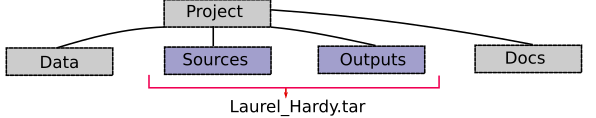
\includegraphics{Figures/architecture.png}
\caption{Exemple de figure: architecture du projet}
\label{fig:2}
\end{center}
\end{figure}

Des figures très soignées ou très jolies impressionnent toujours le lecteur.

Il faut pour cela apprendre à maîtriser les options graphiques des langages comme Matlab ou Python.

 Encore mieux, pour les plus experts, il faut savoir utiliser des logiciels de traitement d'images, comme GIMP par exemple, et des logiciels graphiques vectoriels comme Inkscape. Ces deux logiciels permettent de faire des choses très complexes comme introduire du texte ou des équations dans une figure ou images, ou de superposer des graphes à des images, ou d'autres choses plus complexes. Il faut du temps pour apprendre ces logiciels, mais c'est un investissement rentable pour toute la carrière, en plus des études. 

\subsubsection{Figures en général}

Il existe trois types génériques de figures:
\begin{itemize}
\item des dessins qui illustrent quelque chose, une géométrie, une configuration, une expérience, des mesures,  etc ...
\item des images
\item des graphiques contenant des représentations de résultats numériques sous différentes formes.
\end{itemize}

Parfois une figure est un mélange des trois cas.

Pour tous ces types la figure doit :
\begin{itemize}
\item avoir un numéro  (souvent automatique avec les éditeurs de texte)
\item avoir une légende qui indique clairement le contenu de la figure. La légende peut aller jusqu'à 4 ou 5 lignes parfois, si elle est très descriptive
\item  être centrée sur la largeur de page
\item  avoir une hauteur de 3 à 7 cm. Exceptionnellement elle peut prendre une moitié ou une hauteur totale de page, notamment quand une figure est composé de plusieurs sous-figures.
\item avoir une bonne définition en pixels. Attention aux copies d'écran ou aux images basses définitions qu'on récupère à droite ou à gauche, et qui donne au final un rendu flou
\item respecter le rapport d'aspect de la figure ou image originale. Le rapport d'aspect est le rapport hauteur/largeur. Sinon l'image à l'air d'être étirée dans une direction, ce qui donne un rendu affreux
\item  avoir des  textes  lisible sà l'échelle  100\%, surtout  s'ils sont importants pour comprendre la figure.
\item être positionnée judicieusement dans le document, c'est-à-dire proche de l'endroit où on la décrit. Si ce n'est pas possible, cela indique qu'il n'y a pas assez de commentaires sur les figures et que certaines sont inutiles ou à positionner dans une annexe. 
Deux autres conseils peuvent être donnés:
\begin{itemize}
\item En général on préfère mettre une figure en haut de page ou vers le milieu. 
\item On évite d'avoir une ligne ou deux de texte entre des figures, car en général le lecteur ne les verra pas.
\end{itemize}


\end{itemize}

\subsubsection{Graphiques scientifiques}

Pour les figures représentant des nombres, des fonctions ou  des isolignes ou autre,  il faut veiller à:
\begin{itemize}
\item avoir une légende sur l'axe des abscisses et très très souvent aussi sur l'axe des ordonnées
\item avoir une bonne visibilité des courbes. Cela implique un choix de couleurs, d'épaisseurs ou de taille de symbôles judicieux. 
\item éviter la surcharge de courbe. Au-delà de quelques courbes (3 à 5) on ne voit plus rien sur une figure, sauf si les courbes sont étagées. 
\item avoir une légende pour chaque courbe quand il y en a plusieurs
\item avoir l'échelle des couleurs quand on a des isobarres ou l'échelle des valeurs si possible, quand on a des isolignes.
\item avoir une taille de fonte lisible pour  des nombres et les textes
 sur les axes des abscisses, des ordonnées pour le  titre et les légendes
\item ajouter des lettres lorsqu'on a des sous-figures. Des hauteurs des sous-figures doivent rester décentes (supérieures à 1.5 ou 2 cm). 
\item ce que les échelles sur les deux axes soient choisies judicieusement de manière à ce que le graphique remplisse globalement le cadre. 
\item choisir correctement les axes, en semi log ou log-log ou échelles linéaires
en faisant attention aux signes des valeurs naturellement.
\item  ajouter une grille bien définie si on souhaite prendre des valeurs sur les courbes

\item comparer correctement des résultats lors de validation. On doit avoir par exemple quand c'est possible la courbe résultat et la courbe de référence sur le même graphe, et pas sur deux graphes côte à côte. Lors qu'on est obligé de comparer deux figures côte à côte il faut respecter les dimensions des figures, et avoir des valeurs identiques sur les deux axes, avec une grille.
\end{itemize}

Enfin, quand on fait un commentaire sur une figure, on doit \textbf{faire référence au numéro de la figure}. Le commentaire doit faire quelques lignes. La première chose est de décrire ce qui est représenté. Ensuite on commente les tendances, les variations, les points particuliers (maximun, minimun, discontinuités, ...)

Voici un exemple de commentaire :

La figure \ref{fig:1} représente l'expérience sur un anneau tourbillonnaire (a), un exemple de visualisation à un instant donné(b), et enfin une reconstruction 
de l'anneau tourbillonnaire dans un plan. ... bla bla ...

\bleu{On peut remarque que les nombres sur la figure (c) ont été agrandis et que les épaisseurs des traits sur toutes les figures ont été forcés.}

Deux remarques lorsqu'on veut conserver un graphe pour un rapport ou une présentation:

\begin{itemize}
\item En général dans tous les langages classiques comme Python ou Matlab, les épaisseurs des traits et les hauteurs des nombres par défaut sont optimisées pour la visualisation sur un écran (de grande dimension). Pour une sauvegarde et
une introduction dans un rapport il faut toujours définir les hauteurs et épaisseurs dans le programme et ne pas se contenter des valeurs par défaut. Il faut aussi tenir compte de la possible réduction de l'image dans le document.

\item En toute logique, pour une présentation orale des résultats il faut
refaire des figures spécifiques en augmentant encore la hauteur des textes et l'épaisseur des traits pour améliorer la visibilité via un vidéo-projecteur.
\end{itemize} 

Les figures doivent apparaître dans l'ordre où elles sont nommées. Par exemple ici, je me suis trompé  volontairement en parlant d'abord de la figure \ref{fig:1}
alors que la première à apparaître est la figure \ref{fig:2}.


 
\begin{figure}[htb]
\input{Figures/experiment.pdf_tex}
\caption{Vortex ring experiment and results \cite{Albagnac}, a) experimental set-up,b) example of picture, c) example of the velocity field.}
\label{fig:1}
\end{figure}


 


%**************************
\subsection{Table, tableaux}
%*************************

Les tableaux permettent de synthétiser des résultats numériques ou expérimentaux ou de fournir des paramètres en un coup d'oeil:

\begin{itemize}
\item Il est fortement déconseillé de positionner des tableaux au milieu du texte.
Il vaut mieux les insérer comme des figures avec un numéro et une légende
comme l'exemple du tableau \ref{tab:1}. 

\item Un tableau doit rester sobre. Ainsi sur les deux tableaux présentés
le tableau \ref{tab:1} est largement préférable au tableau \ref{tab:2}.
 
\item On peut ajouter quelques couleurs par alternance, par lignes lorsqu'il y a beaucoup de lignes pour améliorer la lecture et minimiser les erreurs de lecture.

\item Préférer un tableau avec des colonnes larges que des colonnes serrées et  centrer le tableau sur la page.

\end{itemize}

\begin{table}[htb]

\begin{center}
\setstretch{1.5}
\begin{tabular}{c|rrr}
\hline
paramètres / cas & \hs{1.5} $\alpha$ [kg] \hs{1.5} & \hs{1.5} $\beta$ \hs{1.5}  & \hs{1.5} $\gamma$ [mm] \hs{1.5} \\ \hline \hline 
1                & 2.3      & 3.15    & 100.04   \\
2                & 12.3     & 5.20    & 50.10    \\ \hline
\end{tabular}

\setstretch{1}
\end{center}
\caption{Exemple de tableau propre et lisible. Espacements corrects, information complète, alignement des nombres à la virgule. On peut encore enlever la première et la dernière ligne horizontale sur ce tableau.}
\label{tab:1}
\end{table}

\begin{table}[htb]

\begin{center}
\begin{tabular}{|c|c|c|c|}
\hline
paramètres / cas &  $\alpha$  &  $\beta$ & $\gamma$   \\ \hline 
1                & 2.3      & 3.15    & 100.04   \\ \hline
2                & 12.3     & 5.20    & 50.10    \\ \hline
\end{tabular}
\end{center}
\caption{Mauvais exemple de tableau. Trop de traits inutiles, mauvais écartements en vertical et horizontal. Pas d'unité. }
\label{tab:2}
\end{table}

 
 

% *******************************************************
\section{Styles spéciaux}
% *******************************************************

En fonction du contexte on peut appliquer des styles spéciaux pour mettre en avant 
des choses importantes. Il faut rester malgré tout sobre.

  

\Attention{Message d'avertissement avec une mention en anglais.}

 
  \Important{Il faut absolument éviter le plus possible les fautes de grammaire et d'orthographe ainsi que les erreurs typographiques.
  
  Pour cela il faut :
  \begin{itemize}
  \item utiliser les dictionnaires intégrés au logiciel de publication
  \item relire le rapport plusieurs fois, en laissant du temps (heures, jours) entre les lectures.
  \end{itemize}
  
  }
  
  

%***********************************
\section{Conclusion, perspectives}
% **********************************

Quelque soit la rédaction, un document contient nécessairement une introduction et une conclusion.

Pour un compte-rendu, cela est l'occasion de rappeler l'intérêt du TP, ce qu'on a pu apprendre, les difficultés rencontrées et donner par exemple son avis personnel.

On peut ajouter des perspectives.

Pour un compt-rendu,   10 à 15 lignes suffisent amplement.


\vspace{1cm} 
 
La qualité du rapport démontre votre investissement. Un étudiant qui n'a rien compris ou rien fait en TP ne pourra jamais faire un bon rapport. 
Un beau et bon rapport mettra en valeur vos compétences, vos connaissances 
et votre capacité de travail et de compréhension. 
 
\Important{Enfin tout rapport doit contenir une bibliographie, avec des références contenant toutes les informations pour retrouver le document, comme ce qui est fait dans l'exemple ci-dessous.
Cela peut être juste le cours du professeur ou un livre.}

%********************************
\begin{thebibliography}{1}
\bibitem{Albagnac}  Albagnac, J and L\'eard, Pierre and Anne-Archard, D. and Brancher, P. and Cazin, S. and
Rida, Z., \emph{Dynamic of an inclined vortex ring interacting with a density stratification},
Environmental Fluid Dynamics: Confronting Grand Challenges,  2019.
\bibitem{Pinaud} Pinaud, J. and Albagnac, J. and Cazin, S. and Rida, Z. and  Anne-Archard, D. and Brancher, P.,
\emph{Three-dimensional measurements of an inclined vortex ring interacting with a density stratification.}, IMFT report, Toulouse, 2020.
\bibitem{Machin} L. Skywalker, O. Kenobi, \emph{Cours d'astrophysique}, Master 1 Mécanique et Energétique, Université Toulouse III, France, Terre, an 20~010. 
\end{thebibliography}

%*****************
\section{Annexes}
%****************

On peut ajouter une ou deux pages d'annexe. Le format est plus libre car
l'annexe n'est pas toujours lu. On peut avoir par exemple uniquement des figures, ou des équations avec très peu de commentaire.

\subsection{\'Equations du problème}

\vspace{2cm}

\subsection{Figures supplémentaires} 

\vspace{2cm}

\end{document}

     
